\RequirePackage{fix-cm}
\documentclass[11pt,a4paper]{article}
\usepackage[utf8]{inputenc}
\usepackage[T1]{fontenc}
\usepackage{charter}
\usepackage{amsmath,amssymb,amsthm}
\usepackage[margin=0.68in,top=0.62in,bottom=0.62in]{geometry}
\usepackage{graphicx,booktabs,tabularx,array,enumitem,hyperref,xcolor,fancyhdr,microtype,caption,float,lastpage}
\definecolor{primary}{RGB}{27,79,114}
\definecolor{graytext}{RGB}{80,80,80}
\hypersetup{colorlinks=true,linkcolor=primary,citecolor=primary,urlcolor=primary}
\makeatletter
\renewcommand\normalsize{\@setfontsize\normalsize{11.1}{13.3}}
\makeatother
\DeclareMathSizes{11.1}{11.1}{8}{6}
\AtBeginDocument{\normalsize}
\captionsetup{font=normalsize}
\setlength{\parskip}{3pt plus 1pt minus 1pt}
\setlength{\parindent}{0pt}
\setlist{nosep,leftmargin=*}
\setlength{\tabcolsep}{3.2pt}
\renewcommand{\arraystretch}{1.04}
\setlength{\headheight}{14pt}
\setlength{\emergencystretch}{2.5em}
\pagestyle{fancy}
\fancyhf{}
\fancyhead[L]{\fontsize{11.1}{13.3}\selectfont\color{graytext}2026 MCM Senior Track -- Problem B}
\fancyhead[R]{\fontsize{11.1}{13.3}\selectfont\color{graytext}Page \thepage\ of \pageref{LastPage}}
\fancyfoot[C]{\fontsize{11.1}{13.3}\selectfont\color{graytext}Capacity-valid GPU scheduling}
\renewcommand{\headrulewidth}{0.35pt}
\newcommand{\method}[1]{\texttt{#1}}
\newcommand{\takeaway}[2]{\vspace{2pt}\noindent\colorbox{primary!8}{\parbox{\dimexpr\textwidth-2\fboxsep\relax}{\vspace{2pt}\textbf{\color{primary}#1:} #2\vspace{2pt}}}\vspace{2pt}}

\newcommand{\WinnerClaim}{For both FCFS and SPT-HOL, Hash-10\% achieves lower mean A10 JCT at $\sigma=1$, whereas Shape-filtered achieves lower mean A10 JCT at $\sigma=2$. Shape-filtered also has the smaller worst-case value across these two evaluated scenarios.}
\newcommand{\FCFSratio}{27.35}
\newcommand{\BaselineWait}{32.906}
\newcommand{\HashWait}{20.534}

\begin{document}
\begin{center}
{\Large\bfseries\color{primary} Capacity-Valid Scheduling of a Heterogeneous GPU Cluster}\\[3pt]
{\large 2026 HKUST-GZ MCM Senior Track -- Problem B}\\[5pt]
\textbf{Team falcons}\\[3pt]
SHI U Hou, Ziyao Zhang, Beichen Ji, Sirui Zheng\\[3pt]
HKUST(GZ)
\end{center}
\takeaway{Main findings}{In the supplied finite trace, A10 is the main sustained capacity-pressure pool. We use node-level gang checks with SPT-HOL and ratio placement in GS1. HOL strongly benefits multi-worker A10 jobs, while FILL has slightly lower mean waiting for single-worker jobs. GS1 ratio gives zero waiting for all 9,643 jobs in this instance. Under the tested compatibility assumption and $\sigma=1$, dedicating 60 A100 nodes with Hash-10\% routing reduces A10 mean waiting from \BaselineWait{} to \HashWait{} h, with no added native A100 waiting. Slower substitution retains trade-offs, and some A10 jobs finish later. \WinnerClaim{} These conditional choices balance mean delay, tail risk, native harm, and donor occupancy; $\sigma$ is a scenario assumption, not a measured speed.}
\textbf{Data and validation.} We use the supplied 224,112-job trace, exact integer-second durations, six model pools, non-preemptive gang starts, and complete drain for waiting/JCT. Allocation rates use the fixed 90-day window. Original IDs and requested fields, node-level CPU/GPU ledgers, full drain, fixed-window counts, and independently recomputed metrics were checked against saved formal schedules.

\section{Question 1: Workload structure and capacity pressure}
\label{sec:r1q1}
The supplied trace has 224,112 jobs on 4,278 nodes, with 10,412 GPUs and 632,636 vCPUs across six GPU models. For job $j$, $a_j$ is release time, $p_j$ duration, $W_j$ workers, and $(g_j,c_j)$ the per-worker GPU and vCPU requests. Submitted GPU work is $H_j=W_jg_jp_j$; it is a request-based quantity, not measured device utilization. The six model pools have distinct capacities and request shapes; their formal simulated outcomes are reported with the scheduler evidence in Question~2. Supplementary source records identify the exact inputs used for these statistics.

\begin{table}[H]
\centering
\caption{Workload type statistics from the formal raw CSV. Percentages are jobs or submitted GPU-work as labelled; the multi-worker summary reports counts and the median/P95/maximum worker count.}
\label{tab:r2q1types}
\setlength{\tabcolsep}{2.5pt}
\begin{tabularx}{\linewidth}{l>{\raggedright\arraybackslash}X>{\raggedright\arraybackslash}X>{\raggedright\arraybackslash}X}
\toprule
Population & Duration $\le 1$ h (jobs; GPU-work) & Duration $>24$ h (jobs; GPU-work) & Worker structure \\
\midrule
All 224,112 & 70.751\%; 0.721\% & 9.295\%; 92.350\% & $W=1$: 90.953\%; $W>1$: 20,276 jobs (9.047\%). Within multi-worker: $W=2$--8: 16,559; $W\ge9$: 3,717; median/P95/max $=4/28/249$. \\
A10 111,284 & 79.035\%; 0.176\% & 10.717\%; 99.417\% & $W=1$: 99.293\%; $W>1$: 787 jobs (0.707\%). Within multi-worker: $W=2$--8: 637; $W\ge9$: 150; median/P95/max $=4/17.7/60$. \\
\bottomrule
\end{tabularx}
\end{table}

\begin{figure}[H]\centering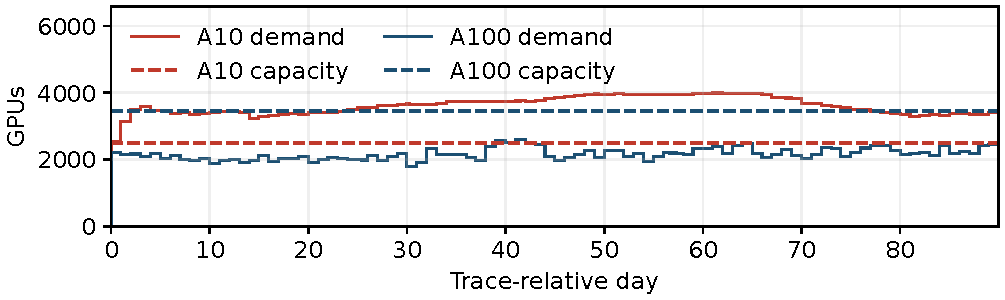
\includegraphics[width=\linewidth]{figures/fig1_demand.pdf}\caption{Exact daily-bin overlap of the immediate-start counterfactual and physical GPU capacity. This is demand/capacity, not simulated allocation. The A10 mean is 3,614.54 GPUs against 2,494 capacity and its peak is 4,103; A100 demand stays below its 3,456-GPU capacity.}\label{fig:r1demand}\end{figure}

The workload is concentrated: GPU-work Gini is 0.9522, the top 1\% (2,241 jobs) contributes 43.30\%, and the top 5\% (11,205 jobs) contributes 87.68\%. Median duration is 1,330 s, the 95th percentile is 309.09 h, and the maximum is about 184 days. There are 3,512 jobs at trace time zero; without a calendar origin, their position is reported as a trace-origin batch rather than a weekday effect. The exposure-corrected relative 24-hour profile peaks at phase hour 16 and is lowest at hour 4 (ratio 2.29); this is a relative phase diagnostic, not a timezone claim.

The shape is also strongly single-worker: 90.95\% of jobs use one worker, 78.42\% use one GPU per worker, and the means are 1.539 workers and 2.003 GPUs per worker. Daily arrivals are nonstationary at the trace scale: the first day contains 8,509 jobs, day 1 contains 5,525, and the minimum is 965 jobs on day 63. These counts describe the observed window and do not identify a calendar effect or a particular arrival process.

\begin{figure}[H]\centering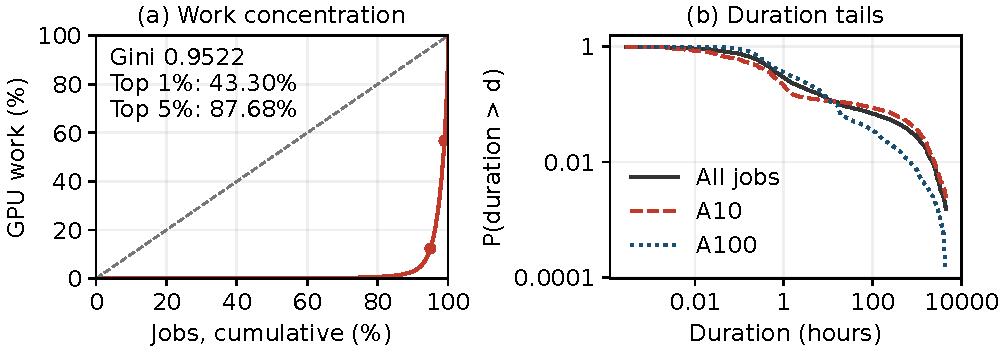
\includegraphics[width=\linewidth]{figures/fig1_data_patterns.pdf}\caption{Two high-information views of the formal data: cumulative GPU-work concentration and strict duration tails.}\label{fig:r1patterns}\end{figure}

For model $m$, with exact Q1 observation window $T=7,775,878$ s, the lifetime-work ratios are
\begin{equation}
\rho_m^{GPU}=\frac{\sum_{j\in\mathcal J_m}W_jg_jp_j}{T\sum_{i\in\mathcal I_m}G_i},\qquad
\rho_m^{CPU}=\frac{\sum_{j\in\mathcal J_m}W_jc_jp_j}{T\sum_{i\in\mathcal I_m}C_i}.
\end{equation}
A10 has $\rho^{GPU}=2.064$, while GPU-series-1 has a shape mismatch: 2,478 jobs (25.70\% of that pool, 78.07\% of its work) exceed the 24-vCPU/GPU ratio of its 8-GPU, 192-vCPU nodes. The 24-, 48-, 128- and 192-vCPU/GPU configurations contain 77, 10, 1 and 901 nodes respectively. This motivates node-level gang checks; it does not identify a unique bottleneck policy.

\section{Question 2: Capacity-valid scheduling}
\label{sec:r2q2}
\subsection{Contract and Algorithm 1}
Each GPU model is simulated as its own pool. A job starts at $s_j\ge a_j$, completes at $f_j=s_j+p_j$, and all $W_j$ workers start together. At a proposed start time, a placement $x_{ji}$ is admitted only if the \emph{pre-start} residual capacities satisfy
\begin{equation}
 g_jx_{ji}\le G_i^{free}(t),\qquad c_jx_{ji}\le C_i^{free}(t),\qquad \sum_i x_{ji}=W_j.
\end{equation}
The resulting full-time model is instead the active-job constraint $\sum_{j:s_j\le t<f_j}g_jx_{ji}\le G_i^{cap}$ and its CPU analogue. Thus a single job's check against residual capacity is not written as a whole-cluster dynamic constraint. Durations are exact integer seconds; gang admission is atomic, non-preemptive and non-migrating.

\takeaway{Algorithm 1 (SPT-HOL)}{For each model pool, insert only arrived jobs into a shortest-processing-time heap keyed by $(p_j,a_j,\mathrm{id}_j)$. Examine the heap head. If it is infeasible on the current residual nodes, stop dispatching this pool at this timestamp (head-of-line blocking). If feasible, scan nodes in the selected placement order, verify every worker slot's GPU and CPU residual, then admit all workers atomically and schedule one completion event. For GPU-series-1 only, the main method uses a CPU/GPU-ratio node order before the same full slot check; every other pool uses ascending-ID first fit. Advance to the next arrival or completion and repeat.}

\method{SPT-FILL} uses the same key but may inspect later feasible jobs under the fixed $K=200$ bypass budget. A heap insertion or removal costs $O(\log n)$; a dispatch also scans candidate nodes and worker slots, and ratio placement orders the candidate nodes by shape. Multiple starts at one timestamp can repeat these scans, so an $O(\log n)$ event claim would be incomplete. Saved schedules were independently checked by route, physical-capacity and metric validators.

The simultaneous-release mechanism has a precise necessary condition. If $f^-$ is the number of free worker slots immediately before an event, $\Delta f$ is the number released by jobs finishing at that event, and $k$ is the next job width, admission requires
\begin{equation}
 f^-+\Delta f\ge k.
\end{equation}
Only with a continuously feasible single-worker backlog and zero free slots after the preceding dispatch does this reduce to $\Delta f\ge k$. A finite $K$ candidate budget can leave $f^->0$, so the reduction is not generally valid. Multiple-worker jobs may wait when free slots cannot accumulate into a gang-sized release; HOL can allow free slots to accumulate while the head is blocked. The formal grouped results in Table~\ref{tab:r2strata} are consistent with this mechanism; it is not the unique proved cause of HOL's result or a starvation-free guarantee.

\begin{table}[H]\centering
\caption{Six-pool SPT-HOL results. GS1 uses ratio; other pools use FF-id. Waiting uses complete drain; allocation and completion use $H=7{,}776{,}000$ s.}
\label{tab:r2pools}
\begin{tabular}{lrrrrrr}
\toprule
Pool & Jobs & GPUs & \shortstack{Mean\\wait (h)} & \shortstack{Median/P99\\wait (h)} & \shortstack{GPU/CPU\\allocation} & \shortstack{90-day\\done}\\
\midrule
A10 & 111,284 & 2,494 & 32.906 & 0.023/1542.181 & 99.922\%/17.927\% & 107,002\\
A100 & 80,877 & 3,456 & 0.000 & 0.000/0.000 & 62.755\%/42.032\% & 80,101\\
GS1 & 9,643 & 1,558 & 0.000 & 0.000/0.000 & 60.867\%/34.814\% & 8,221\\
GS2 & 13,633 & 976 & 0.016 & 0.000/0.045 & 56.931\%/37.424\% & 13,606\\
H800 & 4,716 & 1,752 & 0.016 & 0.000/0.000 & 55.816\%/52.193\% & 4,705\\
A800 & 3,959 & 176 & 0.115 & 0.000/4.390 & 57.311\%/49.493\% & 3,943\\
\bottomrule
\end{tabular}
\smallskip\par A100 and A800 denote the SXM4-80GB models; GS1 and GS2 denote GPU-series-1 and GPU-series-2. Allocation integrates $[0,H)$; a completion at $H$ is included.
\end{table}


The source and configuration mapping for Table~\ref{tab:r2pools} is in the supplement. Exact per-job comparisons confirm that this GS1 placement change leaves A10 timing unchanged.

\subsection{A count lower bound and exact accounting}
For the complete A10 set let $C=2,494$, $G_j=W_jg_j$, $Z(t)=\{j:a_j\le t<a_j+p_j\}$, and let $q(t)$ be the minimum number of jobs removed from $Z(t)$ so that the remaining GPU width is at most $C$. For a schedule, let $S(t)=\{j:s_j\le t<f_j\}$ and $A(t)=S(t)\cap Z(t)$. At any $t$, at least $q(t)$ jobs in $Z(t)$ cannot be simultaneously active, hence $|Z(t)\setminus A(t)|\ge q(t)$. Integrating and using the waiting identity gives
\begin{equation}
\sum_j\min(\omega_j,p_j)=\int |Z(t)\setminus A(t)|\,dt\ge\int q(t)\,dt,
\qquad \sum_j\omega_j\ge\int q(t)\,dt,
\end{equation}
so $L_{count}=(3600N)^{-1}\int q(t)dt=22.3179305700$ h is a lower bound on equal-weight mean waiting. For the observed schedule,
\begin{equation}
\omega_j=\min(\omega_j,p_j)+\max(\omega_j-p_j,0).
\end{equation}
The exact full-A10 accounting, shown with display rounding, is
\begin{equation}
32.9064540350 = 22.3179305700 + 8.3361103922 + 2.2524130728\ \mathrm{h}.
\end{equation}
The first term is the count lower bound, the second is the within-window accounting gap, and the third is waiting beyond a job's own duration. The displayed sum is rounded to the shown precision; these are accounting terms rather than causal shares. The conservative certificates $\bar\omega/L$ are 1.4744 for ordinary job mean and 1.2090 for GPU-work-weighted mean (the latter compares 677.689933 h with the 560.521368 h weighted bound); they are for this fixed instance and different objectives.

\subsection{A10 comparison and worker strata}
For the same complete 111,284-job A10 population and fixed native GPU-work weights $H_j=W_jg_jp_j$, the three formal schedules give:
\begin{table}[H]\centering
\caption{Complete A10 waiting comparison using the same 111,284 jobs and fixed native GPU-work weights.}
\label{tab:r2a10}
\begin{tabular}{lrrrr}
\toprule
Policy & Mean (h) & P99 (h) & Max (h) & \shortstack{GPU-work-weighted\\mean (h)}\\
\midrule
FCFS & 900.129 & 1419.616 & 1423.254 & 619.352\\
SPT-HOL & 32.906 & 1542.181 & 3017.288 & 677.690\\
SPT-FILL & 34.967 & 1575.462 & 3015.311 & 677.496\\
\bottomrule
\end{tabular}

\end{table}


FCFS has lower P99 and maximum waiting than SPT-HOL, but its ordinary mean is \FCFSratio{} times higher; with fixed GPU-work weights, FCFS instead has the lower mean. The supplement identifies the complete formal schedules used in Tables~\ref{tab:r2a10} and~\ref{tab:r2strata}.

SPT-HOL is the average-wait choice on this fixed trace: it lowers ordinary mean waiting by 2.061 h relative to SPT-FILL and lowers P99 by 33.280 h, but its maximum is 1.978 h higher. The management trade-off becomes clearer under the fixed GPU-work objective: the ranking reverses, with SPT-FILL at 677.496 h versus SPT-HOL at 677.690 h. Thus ``lower average but a higher extreme'' and ``different ranking after weighting'' are both observed facts, not dominance claims.

\begin{table}[H]\centering
\caption{HOL/FILL worker strata: waiting in hours; paired difference is HOL minus FILL.}
\label{tab:r2strata}
\begin{tabular}{lrrrrrrr}
\toprule
Stratum & Jobs & \shortstack{HOL\\mean} & \shortstack{FILL\\mean} & \shortstack{HOL\\P99} & \shortstack{FILL\\P99} & \shortstack{Paired\\mean} & \shortstack{Improve / worsen\\/ same (jobs)}\\
\midrule
$W=1$ & 110,497 & 33.125 & 32.805 & 1553.319 & 1539.480 & $+0.320$ & \shortstack{54,489 / 50,566\\ / 5,442}\\
$W=2$--8 & 637 & 1.529 & 186.767 & 15.603$^\dagger$ & 1952.714$^\dagger$ & $-185.237$ & \shortstack{628 / 8\\ / 1}\\
$W\ge9$ & 150 & 4.997 & 982.722 & 36.186$^\dagger$ & 2907.896$^\dagger$ & $-977.725$ & \shortstack{149 / 1\\ / 0}\\
\bottomrule
\end{tabular}
\smallskip\par $^\dagger$ Small strata; P99 is unstable. The groups use the same complete A10 population.
\end{table}


The strata show why a pooled mean can hide policy preference: HOL is much better for multi-worker jobs, whereas FILL has slightly lower mean and P99 for the dominant single-worker stratum. The paired full-trace totals are 55,266 improved, 50,575 worsened and 5,443 unchanged for HOL minus FILL, with mean difference $-2.060576$ h. These values compare the same A10 IDs.

For the fixed GS1 pool, ratio placement is a constructive zero-wait schedule: all 9,643/9,643 jobs have zero waiting and mean waiting 0 h, while the FF-id baselines are 0.029188 h (FCFS) and 0.434277 h (SPT-HOL). Since mean waiting is nonnegative, 0 is the optimum for this fixed GS1 instance. The ratio rule is not generalized to other heterogeneous pools.

\subsection{Second-round policy evidence}
SPT-HEAD-TIME is a bounded policy with a precise implementation definition. When the SPT head is blocked, the code builds a reservation for the first future release event at which the head has a node-level placement witness. While that reservation is active, a backfill candidate is admitted only when it is currently feasible and its finish time is no later than the promised release; a candidate that crosses the promise is rejected by the TIME rule. The $K=200$ budget counts candidate attempts only after the blocked head has started a bypass scan. Under the shared-timer event mode, timer thresholds at each arrival plus $\theta$ create additional dispatch events; for this policy they do not mark jobs urgent. These statements follow the implementation recorded in the supplement, which gives the exact source lines and saved summary.

On the full A10 trace, SPT-HEAD-TIME ($\theta=168$ h, $K=200$, shared timer) changes mean waiting from 32.906454 to 32.923817 h, P99 from 1542.181042 to 1541.586592 h, and maximum from 3017.288056 to 3017.727778 h; its higher cost is not hidden by a single tail statistic. The K/timer and HEAD-TIME results support a bounded mechanism interpretation, not starvation freedom or a general performance theorem. The urgent policies remain prefix-only and are not promoted to the complete-trace recommendation.

\section{Question 3: Fixed-split cross-GPU substitution}
\label{sec:r2q3}
\subsection{Model and two route rules}
A job has native model $n_j$, actual model $m_j$, duration $p_j$, workers $W_j$, and per-worker requests $(g_j,c_j)$. For the sole assumed foreign edge A10$\to$A100-SXM4-80GB, $p'_j=\sigma p_j$; compatibility and $\sigma$ are scenario assumptions, not measured hardware facts. All workers start together on physical nodes, with no migration or preemption, and every start passes the same CPU/GPU slot check.

The no-substitution baseline keeps each job in its native pool. The Hash-10\% rule reserves 60 of 432 A100 nodes for a deterministic 10\% selected A10 subset. The implemented Shape-filtered rule keeps only selected jobs whose CPU/GPU shape fits the donor ratio, yielding 10,604 routed and 605 shape-rejected A10 jobs. It is a fixed physical counterfactual, not a claim that a dynamic policy has been implemented. Source mappings for the main and sensitivity scenarios are in the supplement.

\begin{table}[H]\centering
\caption{Fixed-split results: (a) performance. Waiting and JCT use complete drain; completions use the 90-day horizon.}
\label{tab:q3main}
\begin{tabular}{lrrrrr}
\toprule
Scenario & $\sigma$ & \shortstack{A10 mean\\wait (h)} & \shortstack{A10 mean\\JCT (h)} & \shortstack{All mean\\JCT (h)} & \shortstack{90-day\\completions}\\
\midrule
No substitution & --- & 32.906 & 132.676 & 93.334 & 217,578\\
Hash-10\% & 1 & 20.534 & 120.303 & 87.190 & 217,822\\
Hash-10\% & 2 & 25.106 & 134.810 & 94.393 & 217,529\\
Shape-filtered & 1 & 24.359 & 124.128 & 89.089 & 217,809\\
Shape-filtered & 2 & 24.359 & 129.671 & 91.842 & 217,621\\
\bottomrule
\end{tabular}

\end{table}
\addtocounter{table}{-1}
\begin{table}[H]\centering
\caption{Fixed-split results: (b) harm relative to the No-substitution baseline. A10 harm means a later completion; native A100 harm means increased waiting.}
\label{tab:q3harm}
\begin{tabular}{lrrr}
\toprule
Scenario & $\sigma$ & \shortstack{Native A100\\increased-wait jobs} & \shortstack{A10 later-\\completion jobs}\\
\midrule
No substitution & --- & 0 & 0\\
Hash-10\% & 1 & 0 & 49,772\\
Hash-10\% & 2 & 0 & 56,422\\
Shape-filtered & 1 & 0 & 46,803\\
Shape-filtered & 2 & 0 & 55,465\\
\bottomrule
\end{tabular}
\smallskip\par Both parts use SPT-HOL, GS1 ratio placement, and FF-id in the other pools. Substitution scenarios dedicate 60 A100 nodes to foreign jobs. No substitution keeps the full native pools and has no foreign partition.
\end{table}


\WinnerClaim{} The per-scenario FCFS A10 means are 687.645 versus 756.125 h at $\sigma=1$ and 831.456 versus 761.668 h at $\sigma=2$; for SPT-HOL they are 120.303 versus 124.128 h and 134.810 versus 129.671 h, respectively (Hash-10\% versus Shape-filtered). Thus the two-point maxima are 831.456 versus 761.668 h for FCFS and 134.810 versus 129.671 h for SPT-HOL. These are evaluated points, not an upper bound over an interval, an unknown-speed guarantee, or a unique $\sigma^*$.

\subsection{What the trade-off means}
For SPT-HOL, Hash-10\% is the more aggressive 10\% split; Shape-filtered rejects 605 high-CPU/GPU jobs and changes the selected load. At the tested $\sigma=1$ point, Hash-10\% reduces A10 wait relative to the No-substitution baseline, while Shape-filtered has a smaller A10 benefit but lower paired positive completion-delay mass (16,051.659 job-hours versus Hash-10\% at 68,183.183 job-hours). At $\sigma=2$, common routed-job ordering is unchanged because all durations in one foreign queue are multiplied by the same $\sigma$; re-simulation is still required because completion/release interactions change. Shape-filtered's A10 wait is unchanged at 24.359 h between the two evaluated speeds, but A10 JCT rises 5.542 h and 90-day completions fall by 188.

The A100 allocation uses two explicit denominators. Partition-own rates are computed within each partition: for Hash-10\%, native/foreign are 0.728770/0.682727 at $\sigma=1$ and 0.728770/0.669479 at $\sigma=2$; for Shape-filtered they are 0.728770/0.449232 and 0.728770/0.628414. The full-pool contributions are respectively 0.627552/0.094823, 0.627552/0.092983, 0.627552/0.062393, and 0.627552/0.087280, and each satisfies $U_{\rm all}=(2976U_{\rm native}+480U_{\rm foreign})/3456$, giving 0.722376, 0.720535, 0.689946, and 0.714832. Thus the Shape-filtered foreign partition is 44.923\% allocated and 55.077\% idle at $\sigma=1$, versus 62.841\% allocated and 37.159\% idle at $\sigma=2$; these are partition-own rates and are not full-pool contributions. A larger partition rate is not called a utilization gain by shrinking the native denominator.

The aggregate capacity conversion $534/8=66.75$ is only a pooled arithmetic quantity; it is not rounded to 67 nodes and is not a node-level safe-borrow certificate. The conclusion that 60 donor nodes produce zero native harm is supported by the formal physical schedule, while host safety still depends on node-level placement checks.

\begin{figure}[H]\centering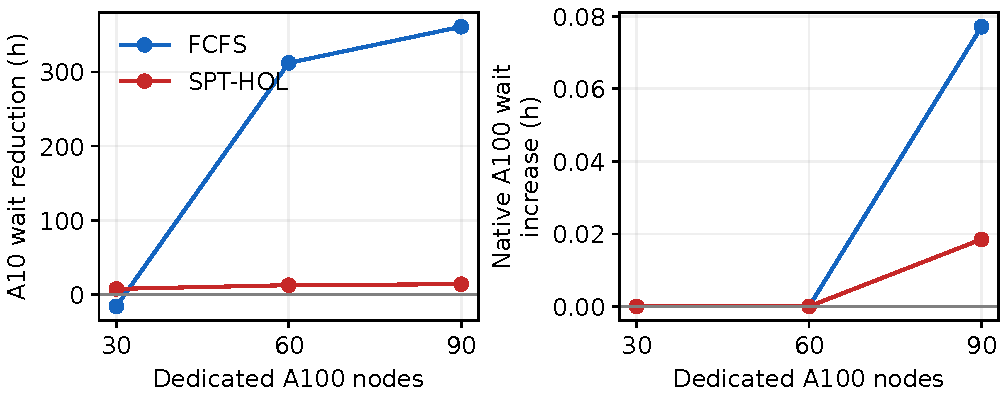
\includegraphics[width=\linewidth]{figures/q3_donor_capacity_wait_tradeoff.pdf}\caption{Donor-capacity sensitivity at 10\% routing and $\sigma=1$, relative to the No-substitution baseline. Left: A10 mean-wait reduction; right: native A100 mean-wait increase. The panels use separate scales.}
\label{fig:r2q3tradeoff}\end{figure}

The sensitivity analysis retains negative cases: at 60 donors, 20\% routing raises FCFS A10 mean wait to 1,010.136 h and its maximum to 5,445.367 h; 30 donors at 10\% gives 916.407 h, worse than No substitution. For the 90-donor case, SPT-HOL native A100 has 2,150 positive-delay jobs, mean additional wait 0.018492 h over all 80,877 native jobs, and harmed-subgroup mean 0.695606 h. These finite paired results expose the management choice between A10 relief, native harm, tail, and completion count.

A financial extension is optional rather than a second experiment. If a tenant values completion time at $v$ per hour and pays $P$, voluntary substitution requires payment reduction at least $v$ times the completion-time increase. No price, participation rate, revenue, or profitability is inferred here. An online completion-cost routing rule remains future work.


\section{Conclusion and limitations}
The three questions answer different decisions. Q1 separates submitted work, immediate-start demand, and simulated allocation. Q2 provides a capacity-valid SPT-HOL contract, a count lower bound, a zero-wait GS1 construction, and complete-A10 tail and cost evidence. Q3 compares fixed physical partitions and evaluated speed assumptions while retaining native harm and duration sensitivity. These are finite trace results: allocation is request occupancy, GPU-hours across models are not interchangeable hardware or monetary units, and no heuristic optimality, speed guarantee, or dynamic substitution policy is claimed. An online completion-cost routing rule remains future work.

\textbf{Strengths and limitations.} Strengths are exact integer-second accounting, node-level CPU/GPU gang checks, saved-ledger replay, and separate ordinary and GPU-work objectives. Limitations are the finite trace, request-based occupancy rather than device telemetry, unbenchmarked cross-GPU compatibility and speed assumptions, and fixed-policy rather than dynamic substitution. The reported choices are conditional on the evaluated cases and do not establish a universal optimum.

\section*{References}
\begin{enumerate}
\item HKUST-GZ MCM 2026 Senior Track, Problem B, ``Scheduling a GPU Cluster,'' official problem statement.
\item Graham, R. L. (1966), ``Bounds on multiprocessing timing anomalies,'' \emph{SIAM Journal on Applied Mathematics}, 14(2), 416--429. Used only as scheduling background; the reported lower bound is derived for this trace.
\item Feitelson, D. G. (2015), \emph{Workload Modeling for Computer Systems Performance Evaluation}. Used for workload-trace terminology and the distinction between demand and allocation.
\item SchedMD, ``Backfill scheduling'' documentation. Used to distinguish a feasible-fill bypass from SPT head-of-line blocking.
\end{enumerate}

\section*{Use of AI Tools}
ChatGPT and OpenAI Codex assisted throughout the research with discussion, program development, data inspection and analysis, mathematical notation, post-processing, evidence and code review, and English writing and typesetting. Claude provided substantive help with candidate lower bounds and decompositions, ratio-placement reasoning, prototype analysis, and cross-review. Formal numerical results come from the team's implemented computations, saved schedules, and independent programmatic validation; AI prototype outputs were not substituted for those results. The team is responsible for checking the content, calculations, code, references, and originality, and for the final submission.
\end{document}
